%\chapter{Importação}
\chapter{Image import}

%O InVesalius importa arquivos no formato DICOM, incluindo arquivos compactados (JPEG sem perdas e
%com perdas) e arquivos no formato Analyze (Mayo Clinic)$^\copyright$.

InVesalius imports files in DICOM format, including compressed files (lossless JPEG), Analyze (Mayo Clinic) $^\copyright$, NIfTI, PAR/REC, BMP, TIFF, JPEG and PNG formats.

\section{DICOM}

%No menu \textbf{Arquivo}, clique na opção \textbf{Importar DICOM...}. Se preferir, use o atalho
%do teclado \textbf{Ctrl + I}. A importação também pode ser acionada pelo ícone da barra de ferramentas
%descrito na figura \ref{fig:import}.

On menu \textbf{File}, click in option \textbf{Import DICOM...}. If you prefer, use the shortcut of keyboard \textbf{Ctrl + I}. Import DICOM images can also be triggered by the toolbar icon described in the figure~\ref{fig:import}.

\begin{figure}[!htb]
\centering

\includegraphics[scale=0.2]{file_import_original.png}
\caption{Shortcut to DICOM import}
\label{fig:import}
\end{figure}

\hspace{.2cm}

%Em seguida, selecione o diretório que contenha os arquivos DICOM, como na figura \ref{fig:win_folder}.
%O InVesalius irá procurar por arquivos também em subdiretórios do diretório escolhido, caso existam. 

Then select the directory containing the DICOM files, as in figure~\ref{fig:win_folder}.
InVesalius will search for files also in subdirectories of the chosen directory, if they exist.


\newpage

%Clique em \textbf{OK}.
Click on \textbf{OK} button.

\begin{figure}[!htb]
\centering
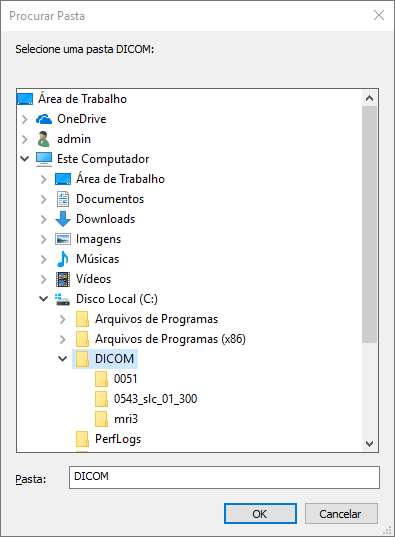
\includegraphics[scale=0.5]{import_select_folder_pt.png}
\caption{Folder Selection}
\label{fig:win_folder}
\end{figure}

\hspace{.2cm}

%Enquanto o InVesalius procura por arquivos DICOM no diretório, é exibido o progresso
%do carregamento dos arquivos verificados, como ilustra a figura \ref{fig:ver_file}.

While InVesalius search for DICOM files in the directory, the loading progress of the scanned files is displayed, as shown in the figure~\ref{fig:ver_file}.

\begin{figure}[!htb]
\centering
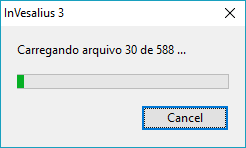
\includegraphics[scale=0.6]{import_load_files_pt.png}
\caption{Checking and loading files status}
\label{fig:ver_file}
\end{figure}

\newpage

%Se arquivos DICOM forem encontrados, é aberta uma janela (figura \ref{fig:win_import})
%para selecionar o paciente e a respectiva série que se deseja abrir. Também é possível
%pular imagens para reconstrução.

If DICOM files are found, a window opens (figure~\ref{fig:win_import}) to select the patient and the respective series to be opened. It is also possible to
skip images for reconstruction.

\begin{figure}[!htb]
\centering
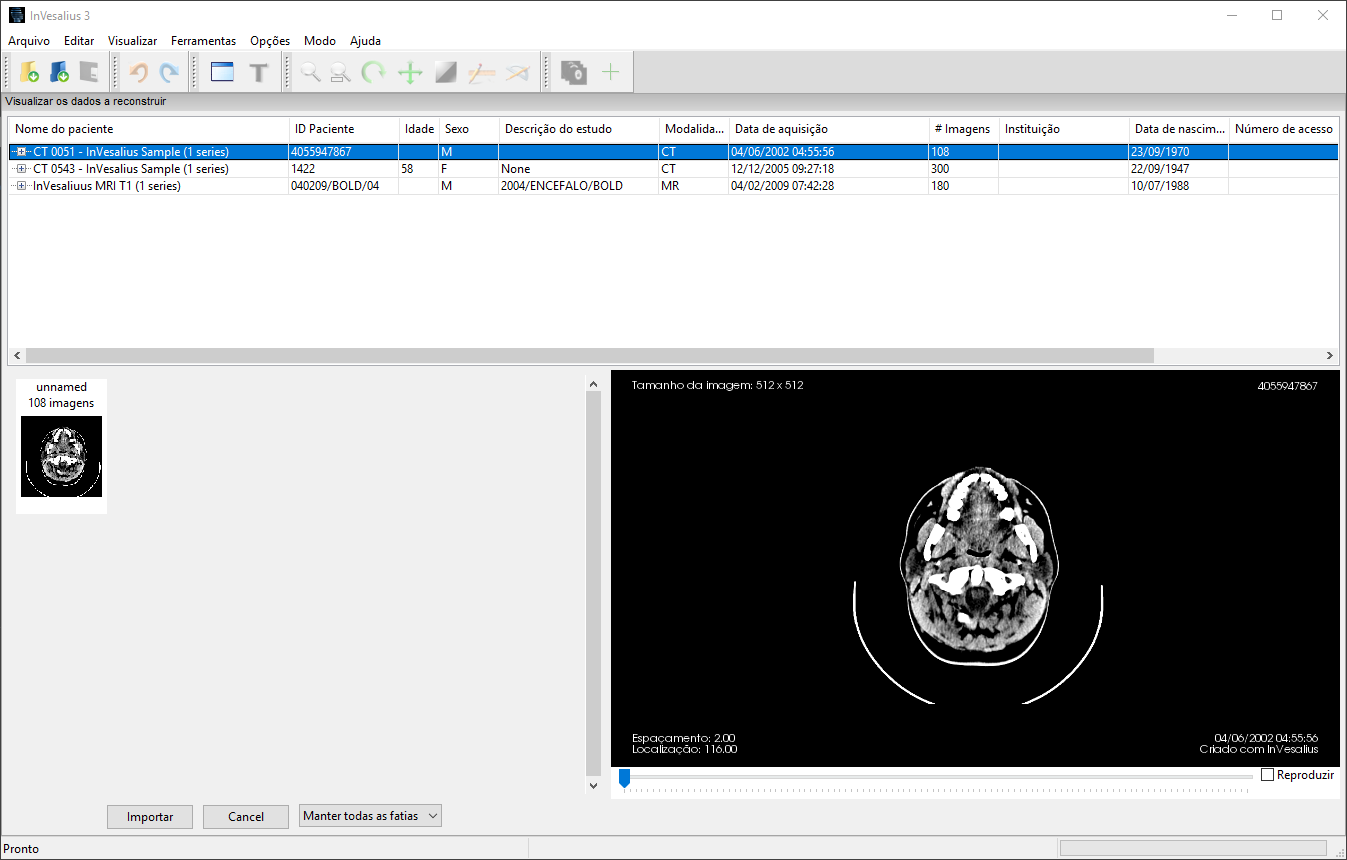
\includegraphics[scale=0.4]{import_window_pt.png}
\caption{Import window}
\label{fig:win_import}
\end{figure}

\newpage



%Caso deseje importar uma série com todas as imagens presentes, clique em "\textbf{+}" ao
%lado do nome do paciente para expandir as séries a ele pertencentes. Dê um \textbf{clique duplo}
%com o botão \textbf{esquerdo} do mouse sobre a descrição da série. Veja a figura
%\ref{fig:import_serie}.


If you want to import a series with all the images present, click "\textbf{+}" in the side patient's name to expand the series belonging to him. \textbf {Double-click} with left mouse button on the description of the series. See figure~\ref{fig:import_serie}.

\begin{figure}[!htb]
\centering
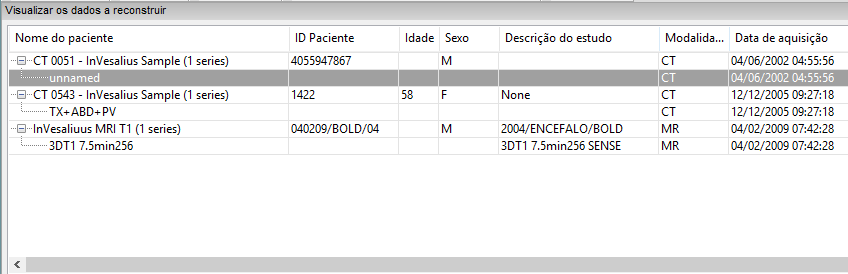
\includegraphics[scale=0.5]{import_window_detail_pt.png}
\caption{Series selection}
\label{fig:import_serie}
\end{figure}
 
%\hspace{.2cm}

%Em alguns casos, em particular quando não se dispõe de um computador com memória e/ou
%processamento satisfatórios para trabalhar com muitas imagens em uma série, pode ser
%recomendável pular (ignorar) algumas delas. Para isso, clique \textbf{uma vez} com o botão
%\textbf{esquerdo} do mouse sobre a descrição da série (figura \ref{fig:import_serie}) e selecione
%quantas imagens serão puladas (figura \ref{fig:skip_image}). Clique em \textbf{Importar}.


In some cases, in particular when there is no computer with memory and/or satisfactory processing to work with many images in a series, can be it is recommended to skip (skip) some of them. To do this, click \textbf {once} with the \textbf{left} of the mouse over the description of the series (figure~\ref{fig:import_serie}) and select how many images will be skipped (figure~\ref{fig:skip_image}). Click~\textbf {Import}.

\begin{figure}[!htb]
\centering
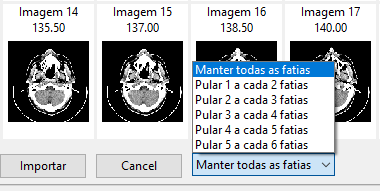
\includegraphics[scale=0.6]{import_window_skip_slice_pt.png}
\caption{Skip imagens}
\label{fig:skip_image}
\end{figure}

%\hspace{.2cm}

%Caso seja detectado quantidade insuficiente de memória disponível na hora de carregar as imagens é recomentado 
%reduzir a resolução das fatias para trabalhar com visualização volumétrica e de superfície, como mostra a janela \ref{fig:resize_image}. 
%As fatias serão redimensionadas de acordo com a porcentagem em relação a resolução original. Por exemplo, 
%se cada fatia do exame contém a dimensão de 512 x 512 pixeis e for sugerido a "Porcentagem da resolução original" em 60\%, 
%cada imagem resultante terá 307 x 307 pixeis. Caso deseje abrir com a resolução original selecione o valor 100.

If insufficient amount of available memory is detected at the time of loading the images it is recommended reduce the resolution of the slices to work with volumetric and surface visualization, as shown in the \ref{fig:resize_image} window.
The slices will be resized according to the percentage relative to the original resolution. For example, if each slice of the exam contains the dimension of 512 x 512 pixels and the "Percentage of original resolution" is suggested to be 60 \%, each resulting image will be 307 x 307 pixels. If you want to open with the original resolution select the value 100.

\begin{figure}[!htb]
\centering
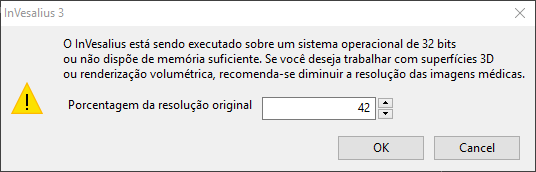
\includegraphics[scale=0.5]{import_window_lower_memory_pt.png}
\caption{Image size reduction}
\label{fig:resize_image}
\end{figure}

%Após os procedimentos anteriores, será apresentada uma janela (figura \ref{fig:prog_recons}) com o progresso
%da reconstrução (quando as imagens são empilhadas e interpoladas).

After the previous procedures, a window will be displayed (figure \ref{fig:prog_recons}) with progress reconstruction (when images are stacked and interpolated).

\begin{figure}[!htb]
\centering
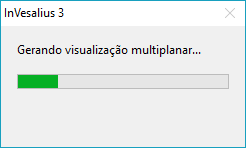
\includegraphics[scale=0.6]{import_window_progress.png} 
\caption{Reconstruction progress}
\label{fig:prog_recons}
\end{figure}

\newpage

\section{Analyze}

%Para importar arquivos no formato Analyze, no menu \textbf{Arquivo}, clique na opção \textbf{Importar outros arquivos...} em seguida a opção \textbf{Analyze} como mostra a figura \ref{fig:analyze_menu}.

To import files in Analyze format, in the menu \textbf{File}, click on \textbf{Importar other files...}, then click in the \textbf{Analyze} option as show the figure~\ref{fig:analyze_menu}.

\begin{figure}[!htb]
\centering
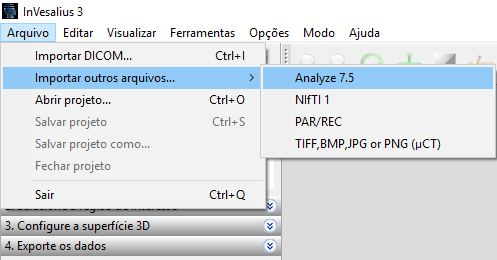
\includegraphics[scale=0.4]{import_analyze_menu_pt.png}
\caption{Menu for importing images in analyze format.}
\label{fig:analyze_menu}
\end{figure}

%Selecione o arquivo do tipo Analyze, na extensão \textbf{.hdr} e clique em \textbf{Abrir}. (figura \ref{fig:analyze_import}).

Select the file of Analyze type, in extension \textbf{.hdr} and click on \textbf{Open}. (Figure \ref{fig:analyze_import}).
 
\begin{figure}[!htb]
\centering
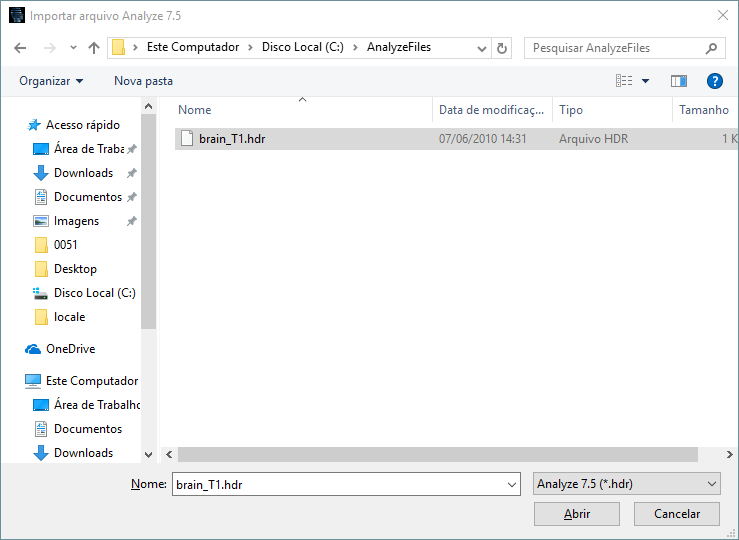
\includegraphics[scale=0.4]{import_analyze_window_pt.png}
\caption{Import analyze file format}
\label{fig:analyze_import}
\end{figure}

\section{NIfTI}

%Para importar arquivos no formato NIfTI, no menu \textbf{Arquivo}, clique na opção \textbf{Importar outros arquivos...} em seguida a opção \textbf{NIfTI} como mostra a figura \ref{fig:import_nifti_menu_pt}.

To import files in NIfTI format, on menu \textbf{File}, click on option \textbf{Import other files...} and then click on \textbf{NIfTI} option as show figure~\ref{fig:import_nifti_menu_pt}.


\begin{figure}[!htb]
\centering
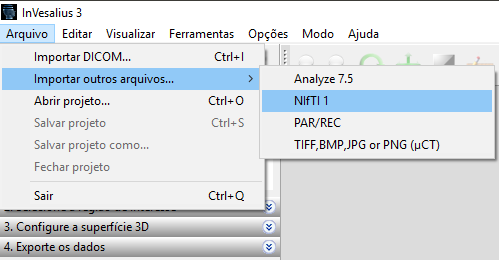
\includegraphics[scale=0.4]{import_nifti_menu_pt.png}
\caption{Menu to import images in NIfTI format}
\label{fig:import_nifti_menu_pt}
\end{figure}

%Selecione o arquivo do tipo NIfTI, na extensão \textbf{nii.gz} ou \textbf{.nii} e clique em \textbf{Abrir}. (figura \ref{fig:import_nifti_window_pt}). Caso o arquivo esteja em outra extensão como \textbf{.hdr}, selecione a opção \textbf{all files(*.*)}.

Select the file of type NIfTI, on \textbf{nii.gz} or \textbf{.nii} extension, click on \textbf{Open} (figure \ref{fig:import_nifti_window_pt}). If the file is in another extension as \textbf{.hdr}, select \textbf{all files(*.*)} option.


\begin{figure}[!htb]
\centering
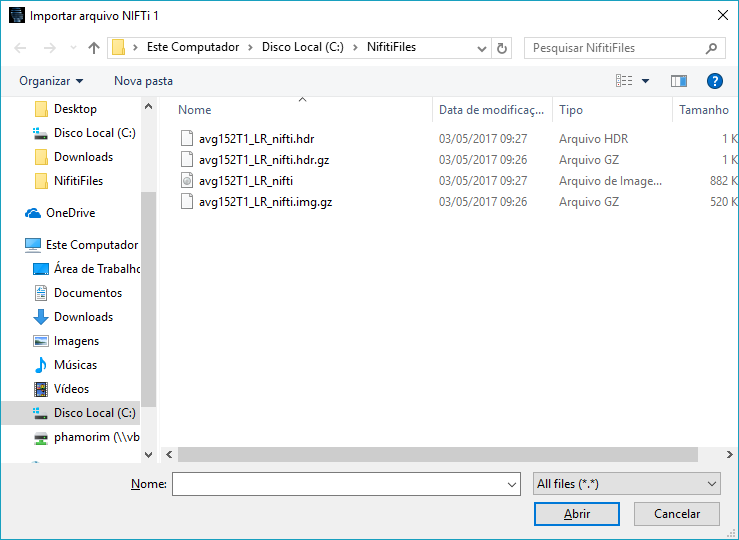
\includegraphics[scale=0.4]{import_nifti_window_pt.png}
\caption{Importing images in NIfTI format.}
\label{fig:import_nifti_window_pt}
\end{figure}

\section{PAR/REC}

%Para importar arquivos no formato PAR/REC, no menu \textbf{Arquivo}, clique na opção \textbf{Importar outros arquivos...} em seguida a opção \textbf{PAR/REC} como mostra a figura \ref{fig:import_parrec_menu_pt}.

To import file in PAR/REC format, on menu \textbf{File}, click on \textbf{Import other files...} option and then click on \textbf{PAR/REC} as shown the figure \ref{fig:import_parrec_menu_pt}.

\begin{figure}[!htb]
\centering
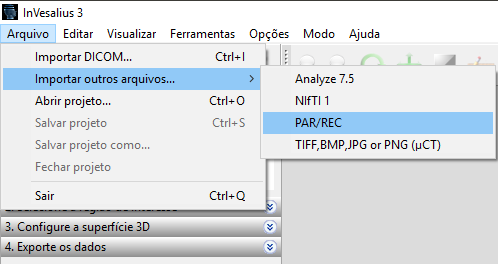
\includegraphics[scale=0.4]{import_parrec_menu_pt.png}
\caption{Menu for importing PAR/REC images}
\label{fig:import_parrec_menu_pt}
\end{figure}

%Selecione o arquivo do tipo PAR/REC, na extensão \textbf{.par} e clique em \textbf{Abrir}. (figura \ref{fig:import_parrec_window_pt}). Caso o arquivo esteja sem extensão, selecione a opção \textbf{all files(*.*)}.

Select PAR/REC file type, in extension \textbf{.par} and click on \textbf{Open} (figure~\ref{fig:import_parrec_window_pt}). If the file has no extension, select \textbf{all files(*.*)} option.

\begin{figure}[!htb]
\centering
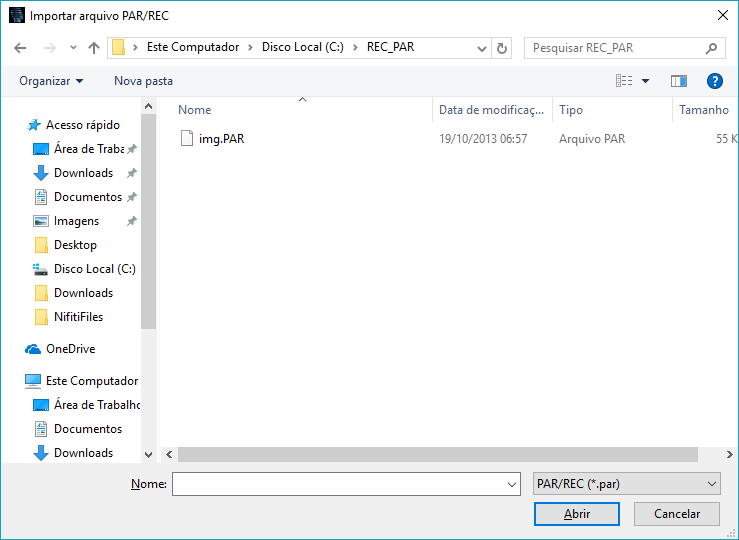
\includegraphics[scale=0.4]{import_parrec_window_pt.png}
\caption{PAR/REC import}
\label{fig:import_parrec_window_pt}
\end{figure}



\section{TIFF, JPG, BMP, JPEG ou PNG (micro-CT)}

%Arquivos em formato TIFF, JPG, BMP, JPEG ou PNG para reconstrução podem ser providos de equipamentos de microtomografia (micro-CT ou $\mu$CT) e outros. O InVesalius importa arquivos nesses formatos desde que os pixels presentes estejam em escala de cinza.

TIFF, JPG, BMP, JPEG or PNG file format for reconstruction can be provided with microtomography equipment (micro-CT or $\mu$CT) or others. The InVesalius imports files in these formats if pixels present are represented in grayscale.


%Para importar, clique no menu \textbf{Arquivo} e na opção \textbf{Importar outros arquivos...} em seguida clique na opção \textbf{TIFF, JPG, BMP, JPEG ou PNG ($\mu$CT)} como mostra a figura~\ref{fig:import_bmp_menu_pt}. 

To import, click on menu \textbf{File}, \textbf{Import other files...} and then click on \textbf{TIFF, JPG, BMP, JPEG ou PNG ($\mu$CT)} option as shown the figure~\ref{fig:import_bmp_menu_pt}.

\begin{figure}[!htb]
\centering
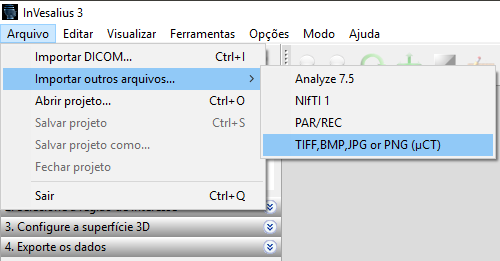
\includegraphics[scale=0.4]{import_bmp_menu_pt.png}
\caption{Import images in BMP and others formats}
\label{fig:import_bmp_menu_pt}
\end{figure}

%Selecione o diretório que contenha os arquivos, como mostra a figura \ref{fig:import_bmp_select_folder}. O InVesalius irá procurar por arquivos também em subdiretórios do diretório escolhido, caso existam.

Select the directory that contains the files, as shown the figure~\ref{fig:import_bmp_select_folder}. InVesalius will search for files also in subdirectories of the chosen directory, if they exist. 

%Clique em \textbf{OK}.

Click on \textbf{OK}.

\begin{figure}[!htb]
\centering
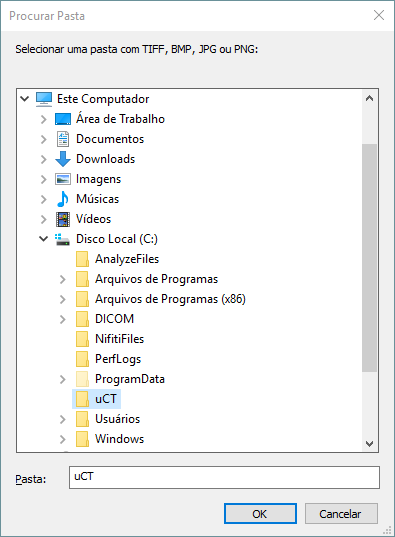
\includegraphics[scale=0.5]{import_bmp_select_folder_pt.png}
\caption{Folder selection}
\label{fig:import_bmp_select_folder}
\end{figure}

%Enquanto o InVesalius procura por arquivos TIFF, JPG, BMP, JPEG ou PNG no diretório, é exibido o progresso do carregamento dos arquivos verificados, como ilustra a figura \ref{fig:import_bmp_load_pt}.

InVesalius searches for TIFF, JPG, BMP, JPEG, or PNG files in the directory, the upload progress of the scanned files is displayed, as illustrated by the \ref{fig:import_bmp_load_pt} figure.

\begin{figure}[!htb]
\centering
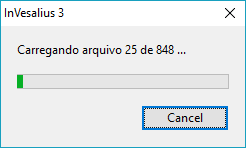
\includegraphics[scale=0.6]{import_bmp_load_pt.png}
\caption{Checking and loading files status.}
\label{fig:import_bmp_load_pt}
\end{figure}

%Se arquivos do tipo TIFF, JPG, BMP, JPEG ou PNG  forem encontrados, é aberta uma janela (figura~\ref{fig:import_bmp_window_pt}) para exibir os arquivos encontrados elegíveis para reconstrução. Também é possível pular imagens para reconstrução ou remover arquivos da lista para reconstrução. Os arquivos são ordenados de acordo com o nome do arquivo, recomenda-se utilizar números em seus nomes de acordo com a ordem que deseja-se obter na reconstrução.

If files of type TIFF, JPG, BMP, JPEG or PNG are found, a window opens (figure~\ref{fig:import_bmp_window_pt}) to display the found files eligible for rebuild. You can also skip images to rebuild or remove files from the rebuild list. The files are sorted according to the file name, it is recommended to use numbers in their names according to the order you want to get in the rebuild.

\begin{figure}[!htb]
\centering
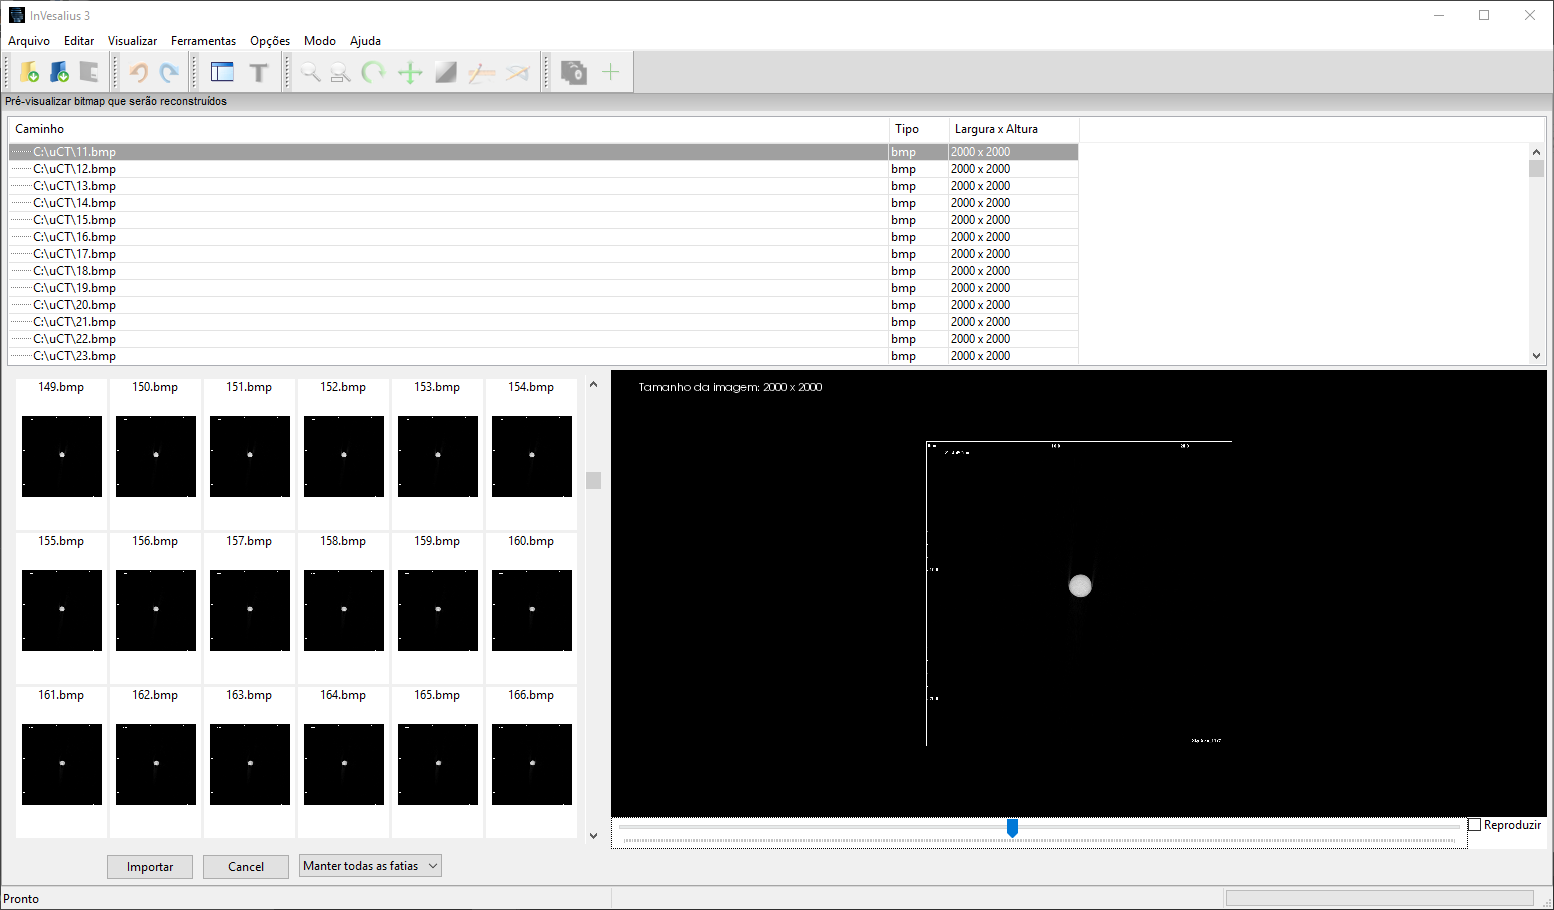
\includegraphics[scale=0.3]{import_bmp_window_pt.png}
\caption{Window to import BMP files.}
\label{fig:import_bmp_window_pt}
\end{figure}

%Para excluir os arquivos que não são de interesse, é possível selecionar um arquivo clicando com o \textbf{botão esquerdo do mouse} e em seguida pressionar a tecla \textbf{delete}. É possível também escolher uma faixa de arquivos para deletar, para isso é necessário clicar com o \textbf{botão esquerdo do mouse} no primeiro arquivo da faixa, manter pressionada a tecla \textbf{shift}, clicar novamente com o \textbf{botão esquerdo do mouse} no último arquivo da faixa e finalmente pressionar o botão \textbf{delete}.
 
To delete files that are not of interest, you can select a file by clicking the \textbf{left mouse button} and then pressing the \textbf{delete} key. You can also choose a range of files to delete, so you need to click the \textbf{left mouse button} on the first file in the track, hold down the \textbf{shift} key, click again with the \textbf{button Left mouse button} in the last file of the track and finally press the \textbf{delete} button.
 
%A exemplo da importação de arquivos DICOM, é possível pular imagens BMP para reconstrução. Em alguns casos, em particular quando não se dispõe de um computador com memória e/ou processamento satisfatórios para trabalhar com muitas imagens em uma série, pode ser recomendável pular (ignorar) algumas delas. Para isso, selecione quantas imagens serão puladas (figura \ref{fig:import_bmp_skip_pt}). Clique em \textbf{Importar}.

Like importing DICOM files module, you can skip BMP images for rebuilding. In some cases, particularly where a computer with satisfactory memory and/or processing is not available to work with many images in a series, it may be advisable to skip (skip) some of them. To do this, select how many images to skip (figure~\ref{fig:import_bmp_skip_pt}). Click \textbf{Import}.

\begin{figure}[!htb]
\centering
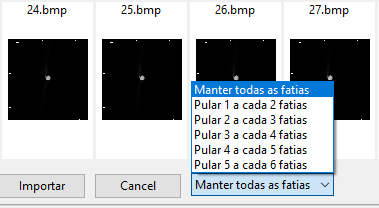
\includegraphics[scale=0.4]{import_bmp_skip_pt.png}
\caption{Importation window}
\label{fig:import_bmp_skip_pt}
\end{figure}

%Para a reconstrução desse tipo de arquivo é necessário definir um nome para o projeto, indicar qual a orientação das imagens (axial, coronal ou sagital), espaçamento do voxel ($X$, $Y$ e $Z$) em \textbf{milímetros} como mostra a figura~\ref{fig:import_bmp_spacing_pt}. O espaçamento do voxel em $X$ é largura do pixel de cada imagem, $Y$ o comprimento do pixel e $Z$ representa a distância de cada fatia (altura do voxel). 

To reconstruct this file type, it is necessary to define a name for the project, to indicate the orientation of the images (axial, coronal or sagittal), voxel spacing ($X$, $Y$ and $Z$) in \textbf{mm} as shown in the figure ~\ref{fig:import_bmp_spacing_pt}. The voxel spacing in $X$ is the pixel width of each image, $Y$ the pixel length, and $Z$ represents the distance of each slice (voxel height).

%Caso o conjunto de imagens seja de imagens de microtomografia, mais especificamente de equipamentos das marcas GE e Brucker, é possível que o InVesalius realize a leitura do arquivo texto com os parâmetros de aquisição que normalmente fica na mesma pasta das imagens e insira automaticamente o espaçamento. Essa constatação pode ser feita quando os valores de $X$, $Y$ e $Z$ são diferentes de "1.00000000", caso contrário é necessário digitar os valores dos respectivos espaçamento. 

If the image set consists of microtomography images, more specifically GE and Brucker equipment, it is possible that InVesalius will read the text file with the acquisition parameters that normally stay in the same folder as the images and automatically insert the spacing . This verification can be done when the values of $X$, $Y$ and $Z$ are different from "1.00000000", otherwise it is necessary to enter the values of the respective spacing.

%\textbf{Atenção, o espaçamento é um parâmetro primordial para a correta dimensão dos objetos no software. Espaçamento incorreto irá fornecer medidas incorretas.}

\textbf{Attention, the spacing is a paramount parameter for the correct dimension of the objects in the software. Incorrect spacing will provide incorrect measurements.}

%Uma vez preenchido todos os parâmetros, basta clicar no botão \textbf{Ok}.
Once you have completed all the parameters, just click the \textbf{Ok} button.


\begin{figure}[!htb]
\centering
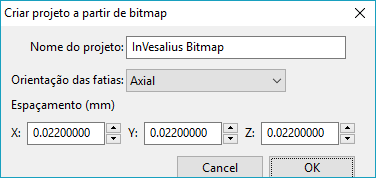
\includegraphics[scale=0.5]{import_bmp_spacing_pt.png}
\caption{Tela de importação}
\label{fig:import_bmp_spacing_pt}
\end{figure}

%Caso seja detectado quantidade insuficiente de memória disponível na hora de carregar as imagens é recomentado  reduzir a resolução das fatias para trabalhar com visualização volumétrica e de superfície, como mostra a janela \ref{fig:import_bmp_resize_pt}.  As fatias serão redimensionadas de acordo com a porcentagem em relação a resolução original. Por exemplo,  se cada fatia do exame contém a dimensão de 512 x 512 pixeis e for sugerido a "Porcentagem da resolução original" em 60\%, cada imagem resultante terá 307 x 307 pixeis. Caso deseje abrir com a resolução original selecione o valor 100.

If insufficient memory is available when loading images, it is recommended to reduce the resolution of the slices to work with volumetric and surface visualization, as shown in the \ref{fig:import_bmp_resize_pt} window. The slices will be resized according to the percentage relative to the original resolution. For example, if each slice of the exam contains the dimension of 512 x 512 pixels and the "Percentage of the original resolution" is suggested at 60\%, each resulting image will have 307 x 307 pixels. If you want to open with the original resolution select the value 100.


\begin{figure}[!htb]
\centering
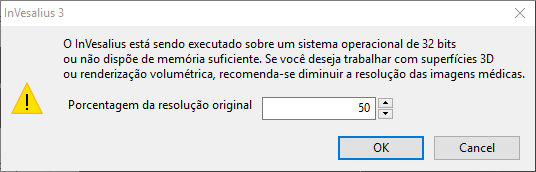
\includegraphics[scale=0.5]{import_bmp_resize_pt.png}
\caption{Image resize}
\label{fig:import_bmp_resize_pt}
\end{figure}

%Após os passos anteriores é necessário aguardar um instante para completar a reconstrução multiplanar conforme mostra a figura~\ref{fig:import_bmp_mpr_pt.png}.

After the previous steps it is necessary to wait a moment to complete the multiplanar reconstruction as shown in the figure~\ref{fig:import_bmp_mpr_pt.png}.

\begin{figure}[!htb]
\centering
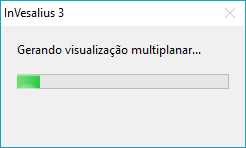
\includegraphics[scale=0.6]{import_bmp_mpr_pt.png}
\caption{Multiplanar reconstruction in progress.}
\label{fig:import_bmp_mpr_pt.png}
\end{figure}